\chapter*{Acknowledgements}

Thanks, as always, to the polycule, who has been endlessly supportive, as well as to Sandy, Kergiby, Kayodé, Rob, Dwale (whose memory is blessed), and many others who helped with reading and keeping me sane along the way.

Thanks also to my patrons:

\begin{description}
    \item[\$10+]
    Donna Karr (thanks, mom); Fuzz Wolf; green; Kit Redgrave; Merry; Orrery; Sandy; Sariya Melody

    \item[\$5]
    Junkie Dawg; Lorxus, an actual fox on the internet

    \item[\$1]
    Alicia Goranson; arc; Katt, sky-guided vulpine friend; Kindar; Muruski; Peter Hayes; Rax Dillon; Ruari
\end{description}

\chapter*{}

\begin{description}
    \item[\emph{Jump}]
    --- Copyright \copyright\ 2021 Madison Scott-Clary

    \item[\emph{Limerent Object}]
    --- Copyright \copyright\ 2021 Madison Scott-Clary

    \item[\emph{Gigs}]
    --- Copyright \copyright\ 20202 Madison Scott-Clary

    "Gigs" appeared on the Voice of Dog podcast.

    \item[\emph{Sorting Laundry}]
    --- Copyright \copyright\ 2017 Madison Scott-Clary

    \item[\emph{Morning Of}]
    --- Copyright \copyright\ 2021 Madison Scott-Clary

    \item[\emph{Foxes and Milkshakes}]
    --- Copyright \copyright\ 2021 Madison Scott-Clary

    A version of "Foxes and Milkshakes" appeared in the Further Confusion 2015 con book and on the Voice of Dog podcast.
\end{description}
\newpage
\thispagestyle{empty}
\null
\vfill

\begin{center}
  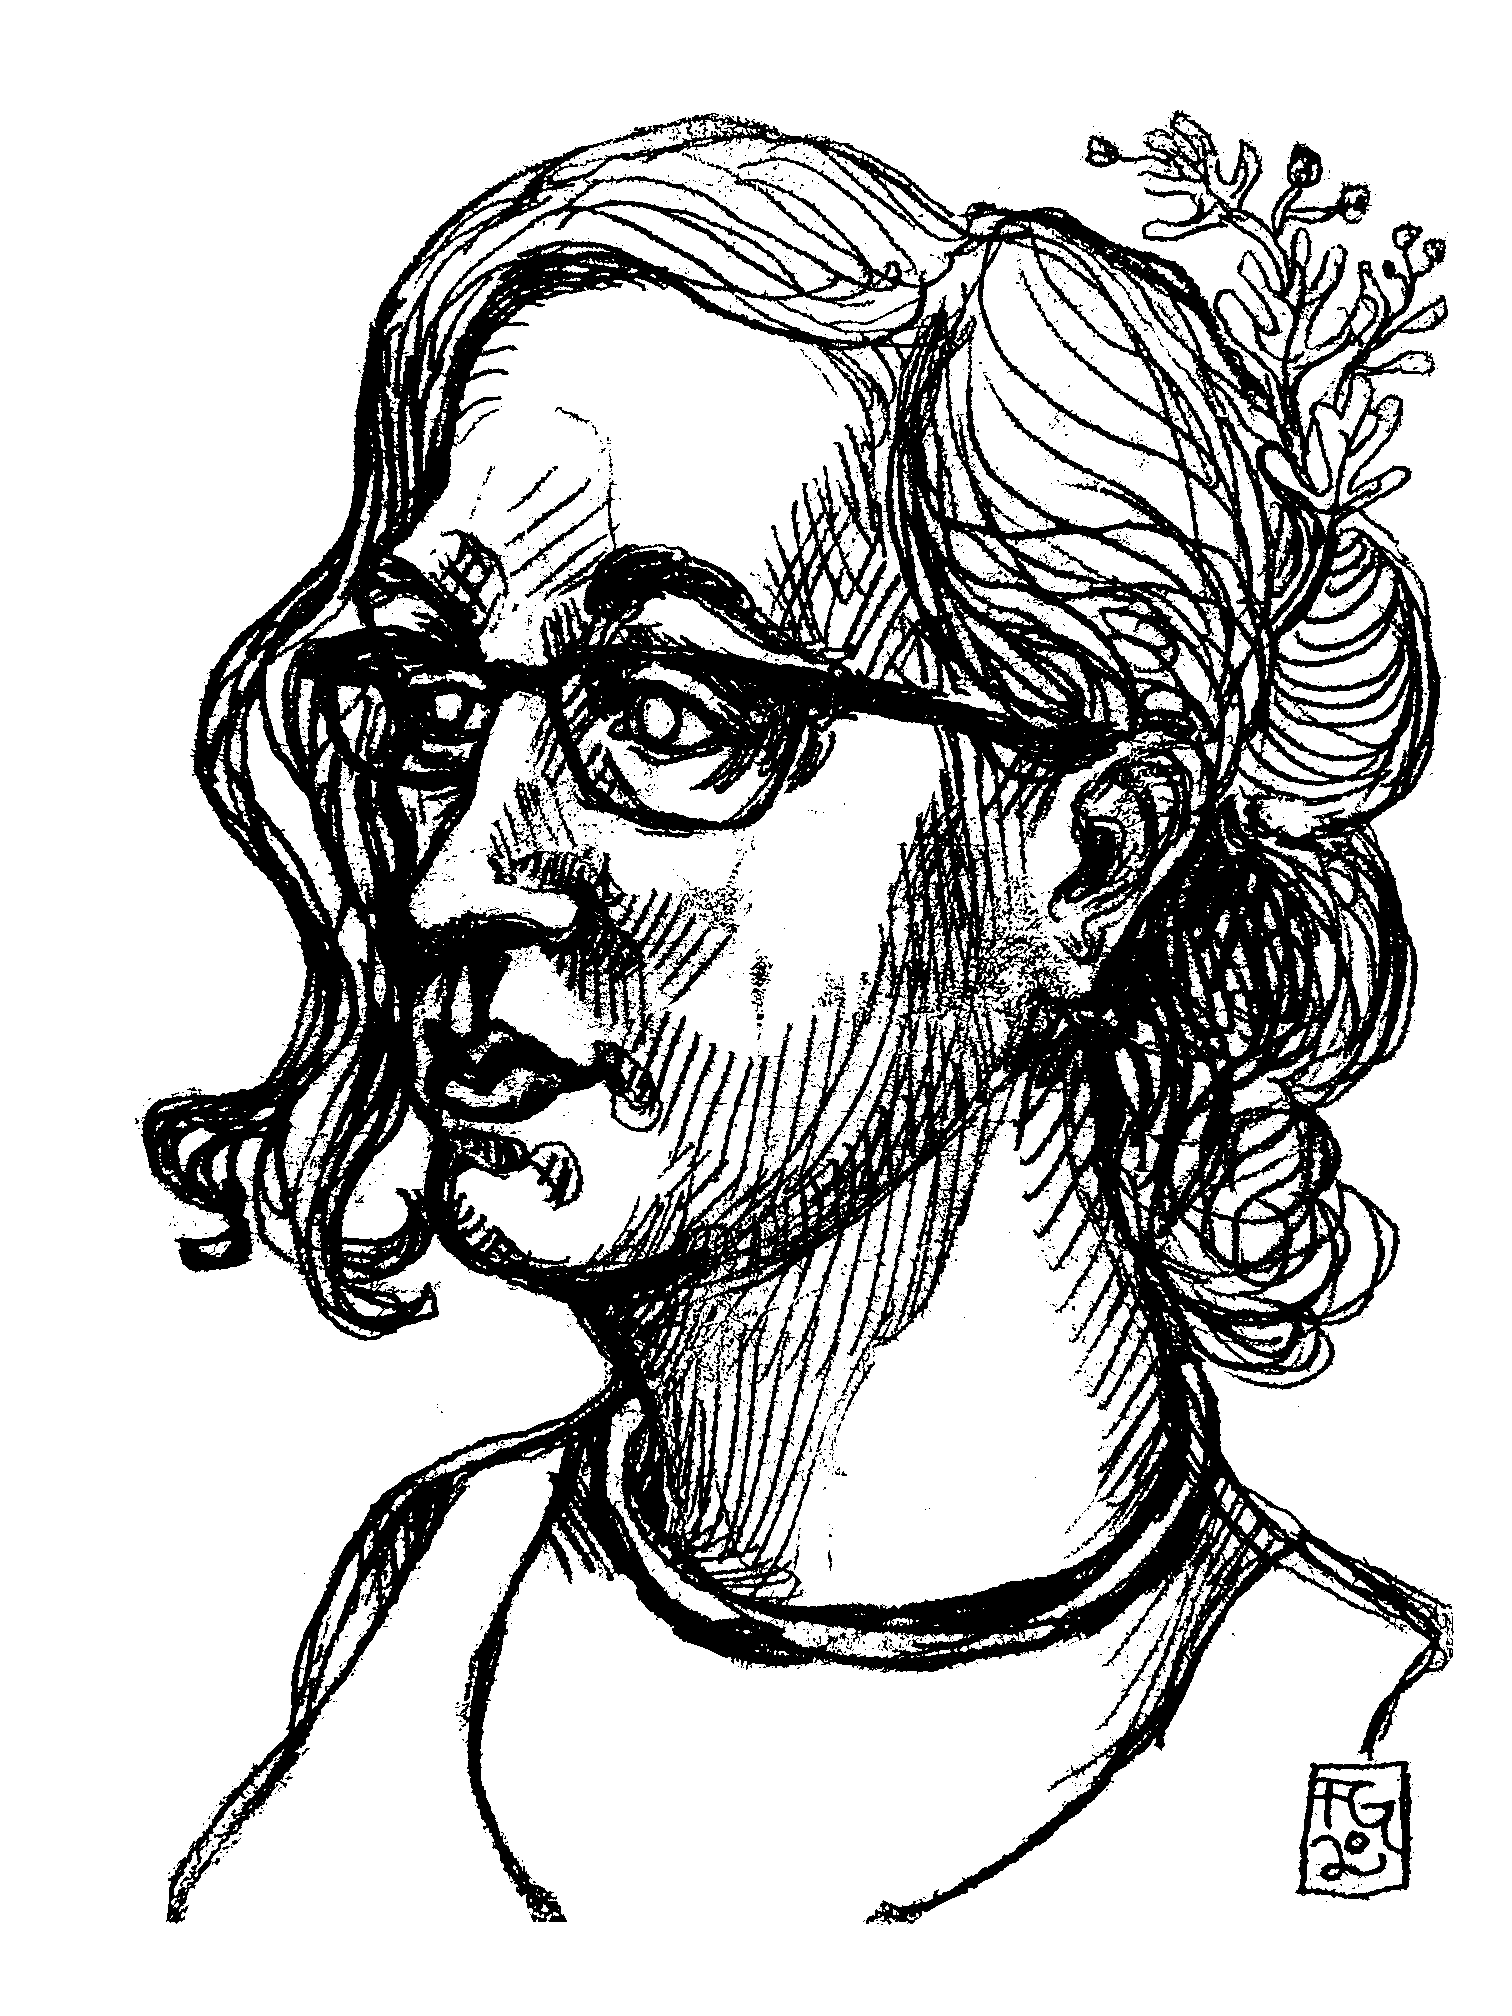
\includegraphics[width=2in]{content/headshot.png}
\end{center}

\noindent Madison Scott-Clary is a transgender writer, editor, and software engineer. She focuses on furry fiction and non-fiction, using that as a framework for interrogating the concept of self and exploring across genres. A graduate of the Regional Anthropomorphic Writers Workshop in 2021, hosted by Kyell Gold and Dayna Smith, she is studying creative writing at Cornell College in Mount Vernon, IA. She lives in the Pacific Northwest with her cat and two dogs, as well as her husband, who is also a dog.

\begin{center}
    www.makyo.ink
\end{center}

\vfill
